\section*{1. Kepler's laws}

a) State the three laws of Kepler\\
\\
\textbf{1. Law of ellipses:} Bodies move around a body with way greater mass in an ellipitcal path and
the greater body being at one of the focal points of the ellipses.\\
\\
\textbf{2. Law of equal areas:} The body moving around the other doesn't move with a constant velocity 
around in the ellipitcal path as it covers always the same area that is drawn on the ellipses in the same 
time, meaning if the body is further away from the focal point it moves slower as it would when it is 
close to it.\\
\\
\textbf{3. Law of harmonic time:} The planet's orbital period is proportional to the cube of the length
of the semi-major axis of the ellipses.\\
\\
b) The comet Tschurjumow-Gerassimenko has a perihelion of 1.21 AU and an orbital period of 6.43 yr. What 
is the aphelion of the comet's orbit? Give the answer in both AU and in km.\\
\\
With Kepler's third law we can determine the lenght of the semi-major axis since the orbital period is 
given:
\begin{equation*}
    \begin{split}
        \frac{a^3}{T^2} &= \frac{G(M + m)}{4 \pi^2} \approx \frac{GM}{4 \pi^2}\\
        a^3 &= \frac{GMT^2}{4 \pi^2}\\
        a &= \sqrt[3]{\frac{GM}{4 \pi^2} \cdot T^2}\\
          &= \sqrt[3]{\frac{T^2}{yr^2}} \cdot \sqrt[3]{\frac{GM}{4 \pi^2} \cdot yr^2}\\
    \end{split}
\end{equation*}
The term $\sqrt[3]{\frac{GM}{4 \pi^2} \cdot yr^2}$ is the definition of the astronomical unit $AU$, which
is why we receive:
\begin{equation*}
    \begin{split}
        a &= \sqrt[3]{\frac{T^2}{yr^2}} AU\\
          &= \sqrt[3]{\frac{6.43^2 \cdot yr^2}{yr^2}} AU\\
          &= \sqrt[3]{6.43^2} AU\\
            &\approx 3.4579 AU\\
    \end{split}
\end{equation*}
The aphelion we receive by subtracting the perihelion from the full major axis:
\begin{equation*}
    \begin{split}
        d_{aphelion} &= 2a - d_{perihelion}\\
        &= 2a - d_{perihelion}\\
        &= 2 \cdot 3.4579 AU - 1.21 AU\\
        &= 5.7058 AU\\
        &= 5.7058 \cdot 1,496e+8 km\\
        &\approx 8,535755e+12 km\\
    \end{split}
\end{equation*}
c) This and next year's spring equinox happend on March 20, while this year's fall equinox occured on
September 22. If you count the days, there are roughly 186 days between the spring and fall equinox, but
only 179 days between fall and the next spring equinox. Using Kepler's laws, explain why the nothern 
winter seems to take less time than the northern summer. During which season is the Earth closer to the 
Sun?\\
\\
An equinox occurs when the Sun's declanation is $0 \degree$. The Earth's axis is tilted in perspective to
the Sun. Also the orbital eccentricity of the Earth is about 0.017, which means that the Sun is at one of
the foci and there is aphelion and perihelion which the Earth reaches. The two equinox points draw a line
throught the ellipses of Earth's orbit deviding the ellipses in a not mirror symmetrical but symmetrical
manner. That means that the two lengths which we receive from the circumference are equal. The perihelion
and aphelion are each on one of these lengths. Due to Kepler's second law these to lengths will be run
with two different velocities, one being faster and one slower. Due to the slight ellipitcal shape of the
orbit this difference will be noticed in only a few days as stated in the problem setting.\\
\noindent\makebox[\textwidth]{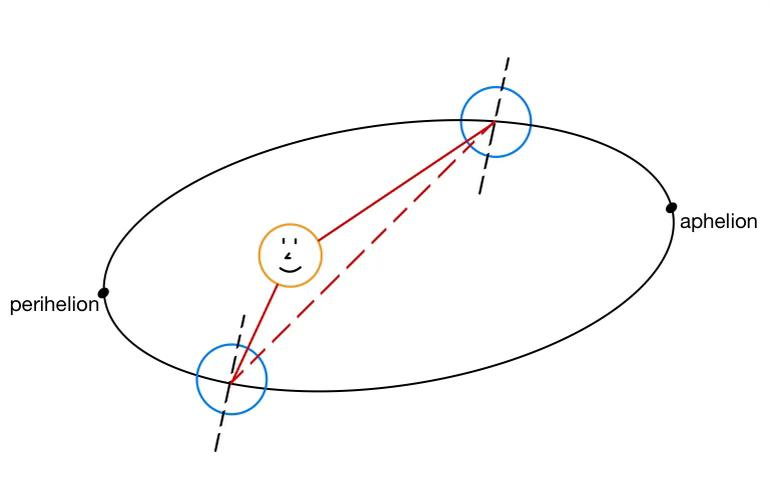
\includegraphics[scale=0.35]{orbit.jpeg}}
\noindent
During the northern winter the Earth is closer to the Sun, which means that the Earth has a higher 
velocity on it's circular path and which is why this season takes less time.
